% !TEX program = xelatex
% Compile with XeLaTeX or LuaLaTeX (run 3 times so the TOC / lists settle):
%     xelatex UROP_report.tex
% Needs srm-logo.png (SRM University-AP emblem) in the same folder.
\documentclass[12pt,a4paper]{article}

%% ------------------------------------------------------------------
%% Page geometry
%% ------------------------------------------------------------------
\usepackage[a4paper,top=1in,bottom=1in,left=1in,right=1in,
            headheight=15pt,headsep=0.3in,footskip=0.45in]{geometry}

%% ------------------------------------------------------------------
%% Fonts: Book Antiqua (TeX Gyre Pagella fallback); LM Mono for code
%% ------------------------------------------------------------------
\usepackage{fontspec}
\IfFontExistsTF{Book Antiqua}{%
  \setmainfont{Book Antiqua}%
}{%
  \setmainfont{TeX Gyre Pagella}%
}
\setmonofont{Latin Modern Mono}[Scale=0.92]
\usepackage{microtype}

%% ------------------------------------------------------------------
%% Packages
%% ------------------------------------------------------------------
\usepackage{xcolor}
\usepackage{setspace}
\usepackage{graphicx}
\usepackage{enumitem}
\usepackage{booktabs}
\usepackage{tabularx}
\usepackage{colortbl}
\usepackage{amsmath,amssymb}
\usepackage[hyphens]{url}
\usepackage{fancyhdr}
\usepackage{titlesec}
\usepackage[titles]{tocloft}
\usepackage[font=small,labelfont={bf,color=navy},labelsep=period,
            skip=8pt]{caption}
\usepackage{tikz}
\usetikzlibrary{arrows.meta,shapes.geometric,calc}

%% ------------------------------------------------------------------
%% Colours
%% ------------------------------------------------------------------
\definecolor{navy}{HTML}{1F3A5F}
\definecolor{rulegray}{HTML}{8A8F98}

%% ------------------------------------------------------------------
%% Paragraph formatting
%% ------------------------------------------------------------------
\setstretch{1.12}
\setlength{\parindent}{0pt}
\setlength{\parskip}{7pt}
\raggedbottom
\tolerance=1000
\emergencystretch=2em
\widowpenalty=10000
\clubpenalty=10000

\setlist[enumerate]{leftmargin=2em,itemsep=3pt,topsep=2pt,parsep=0pt,label=\arabic*.}
\setlist[itemize]{leftmargin=2em,itemsep=3pt,topsep=2pt,parsep=0pt,label=\textbullet}

%% ------------------------------------------------------------------
%% Headings
%% ------------------------------------------------------------------
\titleformat{\section}
  {\color{navy}\fontsize{18pt}{22pt}\selectfont\bfseries}
  {\thesection}{0.7em}{}
  [{\vspace{-2pt}\color{navy}\titlerule[0.8pt]}]
\titleformat{\subsection}
  {\color{navy}\fontsize{13pt}{16pt}\selectfont\bfseries}
  {\thesubsection}{0.6em}{}
\titleformat{\subsubsection}
  {\color{navy}\fontsize{12pt}{15pt}\selectfont\bfseries\itshape}
  {\thesubsubsection}{0.6em}{}
\titlespacing*{\section}{0pt}{0pt}{16pt}
\titlespacing*{\subsection}{0pt}{14pt}{3pt}
\titlespacing*{\subsubsection}{0pt}{10pt}{2pt}

%% ------------------------------------------------------------------
%% Header and footer
%% ------------------------------------------------------------------
\pagestyle{fancy}
\fancyhf{}
\fancyhead[L]{\small\itshape ElseWhere -- UROP Project Report}
\fancyhead[R]{\small\itshape SRM University -- AP}
\fancyfoot[C]{\small\thepage}
\renewcommand{\headrulewidth}{0.4pt}
\renewcommand{\headrule}{\hbox to\headwidth{\color{rulegray}\leaders\hrule height \headrulewidth\hfill}}
\renewcommand{\footrulewidth}{0pt}
\fancypagestyle{plain}{\fancyhf{}\renewcommand{\headrulewidth}{0pt}\fancyfoot[C]{\small\thepage}}

%% ------------------------------------------------------------------
%% Table of contents / lists
%% ------------------------------------------------------------------
\renewcommand{\cftsecfont}{\bfseries}
\renewcommand{\cftsecpagefont}{\bfseries}
\renewcommand{\cftsecleader}{\bfseries\cftdotfill{\cftdotsep}}
\renewcommand{\cftdotsep}{1.5}
\setlength{\cftbeforesecskip}{4pt}
\setlength{\cftbeforesubsecskip}{0pt}
\setlength{\cftsecindent}{0pt}
\setlength{\cftsecnumwidth}{2.2em}
\setlength{\cftsubsecindent}{2.2em}
\setlength{\cftsubsecnumwidth}{2.8em}
\setlength{\cftbeforefigskip}{3pt}
\setlength{\cftbeforetabskip}{3pt}
\setlength{\cftfignumwidth}{2.8em}
\setlength{\cfttabnumwidth}{2.8em}

%% ------------------------------------------------------------------
%% Links
%% ------------------------------------------------------------------
\usepackage[hidelinks,
            pdftitle={ElseWhere: High-Performance Local-First Collaborative LaTeX and AI-Assisted Research Authoring Platform},
            pdfauthor={Venkatesh Konnipati}]{hyperref}
\urlstyle{same}

%% ------------------------------------------------------------------
%% Helper macros
%% ------------------------------------------------------------------
\newcommand{\code}[1]{\texttt{#1}}
\newcommand{\emptypara}{\mbox{}\par}

% Unnumbered front-matter / back-matter section that still appears in the TOC
\newcommand{\frontsection}[1]{%
  \clearpage\phantomsection
  \addcontentsline{toc}{section}{#1}%
  \section*{#1}}

% Table column types
\newcolumntype{L}{>{\raggedright\arraybackslash}X}
\newcolumntype{C}{>{\centering\arraybackslash}X}
\newcolumntype{H}{>{\columncolor{navy!7}\centering\arraybackslash}X}

%% ------------------------------------------------------------------
%% TikZ styles for the figures
%% ------------------------------------------------------------------
\tikzset{
  layer/.style={draw=navy, fill=navy!8, rounded corners=3pt, thick,
                align=center, text width=11.6cm, minimum height=1.15cm,
                inner sep=4pt},
  half/.style={draw=navy, fill=navy!8, rounded corners=3pt, thick,
               align=center, text width=5.4cm, minimum height=2.5cm,
               inner sep=4pt},
  stepbox/.style={draw=navy, fill=navy!8, rounded corners=3pt, thick,
               align=center, text width=4.2cm, minimum height=1.25cm,
               inner sep=4pt},
  goodbox/.style={draw=navy, fill=navy!22, rounded corners=3pt, thick,
                   align=center, text width=4.2cm, minimum height=1.25cm,
                   inner sep=4pt},
  decision/.style={draw=navy, fill=white, diamond, aspect=2.4, thick,
                   align=center, inner sep=1pt, text width=1.9cm},
  arr/.style={-{Stealth[length=2.6mm]}, thick, color=navy},
  lbl/.style={font=\scriptsize\itshape, text=black!70, align=left, inner sep=2pt},
}

\begin{document}

%% ==================================================================
%%  TITLE PAGE
%% ==================================================================
\thispagestyle{empty}
\begin{center}
\setstretch{1.0}
\vspace*{0.1in}

\includegraphics[width=4.2cm]{srm-logo.png}\par
\vspace{0.3in}
{\color{navy}\fontsize{12pt}{15pt}\selectfont\bfseries SRM University -- AP, Andhra Pradesh}\par
{\color{navy}\small School of Engineering and Sciences}\par

\vfill
{\color{navy}\rule{0.55\textwidth}{1.2pt}}\par
\vspace{14pt}
{\color{navy}\fontsize{30pt}{36pt}\selectfont\bfseries ElseWhere}\par
\vspace{8pt}
{\fontsize{15pt}{20pt}\selectfont\bfseries High-Performance Local-First Collaborative \LaTeX{}\\
\& AI-Assisted Research Authoring Platform\par}
\vspace{14pt}
{\color{navy}\rule{0.55\textwidth}{1.2pt}}\par

\vfill
{\fontsize{12pt}{16pt}\selectfont
UROP Project Report submitted to\par
SRM University -- AP, Andhra Pradesh\par
for the partial fulfillment of the requirements for the award of the degree of\par}
\vspace{10pt}
{\fontsize{14pt}{18pt}\selectfont\bfseries Bachelor of Technology\par}
{\fontsize{12pt}{16pt}\selectfont in\par}
{\fontsize{14pt}{18pt}\selectfont\bfseries Computer Science and Engineering\par}

\vfill
\begin{minipage}[t]{0.46\textwidth}
\centering
{\color{navy}\small\bfseries\scshape Submitted by}\par\vspace{4pt}
\textbf{Venkatesh Konnipati (Project Creator)}\par
AP23110011492
\end{minipage}\hfill
\begin{minipage}[t]{0.46\textwidth}
\centering
{\color{navy}\small\bfseries\scshape Under the Guidance of}\par\vspace{4pt}
\textbf{Dr.\ Sanjay Kumar}\par
Assistant Professor\par
Department of Computer Science and Engineering
\end{minipage}

\vfill
{\fontsize{11pt}{14pt}\selectfont
\textbf{SRM University -- AP}\par
Neerukonda, Mangalagiri, Guntur, Andhra Pradesh -- 522\,240\par
\textbf{November, 2026}\par}
\vspace*{0.1in}
\end{center}

%% ==================================================================
%%  FRONT MATTER (roman numerals)
%% ==================================================================
\clearpage
\pagenumbering{roman}
\setcounter{page}{1}

%% ---------------- Bonafide certificate ----------------
\phantomsection
\addcontentsline{toc}{section}{Bonafide Certificate}
\section*{Bonafide Certificate}

\noindent This is to certify that the Undergraduate Research Opportunities Program (UROP) project report entitled \textbf{``ElseWhere: High-Performance Local-First Collaborative \LaTeX{} \& AI-Assisted Research Authoring Platform''} submitted by \textbf{\mbox{Venkatesh Konnipati}} (Registration No.: \textbf{AP23110011492}) to the Department of Computer Science and Engineering, SRM University -- AP, Andhra Pradesh, for the partial fulfillment of the requirements for the award of the degree of \textbf{Bachelor of Technology in Computer Science and Engineering}, is a bonafide record of the research and development work carried out by him under my supervision and guidance.

\noindent To the best of my knowledge, the matter embodied in this report has not been submitted to any other university or institute for the award of any degree or diploma.

\vspace{2.2in}
\noindent
{\small\hyphenpenalty=10000\exhyphenpenalty=10000
\begin{tabular}{@{}>{\raggedright\arraybackslash}p{0.47\textwidth}@{\hspace{0.06\textwidth}}>{\raggedright\arraybackslash}p{0.47\textwidth}@{}}
\rule{0.85\linewidth}{0.4pt} & \rule{0.85\linewidth}{0.4pt} \\[3pt]
\textbf{Dr.\ Sanjay Kumar} & \textbf{Head of the Department} \\
Project Guide & Department of Computer Science \& Engineering \\
Assistant Professor & School of Engineering and Sciences \\
Department of Computer Science \& Engineering & SRM University -- AP \\
SRM University -- AP & Andhra Pradesh -- 522\,240 \\
\end{tabular}}

%% ---------------- Acknowledgements ----------------
\frontsection{Acknowledgements}

\noindent I would like to express my sincere gratitude and deep respect to my project guide, \textbf{Dr.\ Sanjay Kumar}, Assistant Professor, Department of Computer Science and Engineering, SRM University -- AP, for his continuous guidance, constructive feedback, and invaluable encouragement throughout the conceptualization, system architecture design, and implementation of the \textbf{ElseWhere} platform. His technical insights and support pushed me to maintain rigorous engineering standards and complete this research project within the designated timeframe.

\noindent I express my heartfelt gratitude to the faculty and administration of the \textbf{Department of Computer Science and Engineering} and the \textbf{School of Engineering and Sciences}, SRM University -- AP, for providing state-of-the-art computational infrastructure, laboratories, and an inspiring academic atmosphere that fosters student research and innovation.

\noindent Finally, I convey my deepest appreciation to my family, mentors, and peers whose encouragement, patience, and unwavering belief in my abilities sustained my dedication and focus throughout this research endeavor.

\vspace{0.8in}
\begin{flushright}
\setstretch{1.0}
\textbf{Venkatesh Konnipati}\\
Registration No.: AP23110011492\\
Department of Computer Science and Engineering\\
SRM University -- AP
\end{flushright}

%% ---------------- Table of contents ----------------
\clearpage
\renewcommand{\contentsname}{Table of Contents}
\tableofcontents

%% ---------------- Abstract ----------------
\frontsection{Abstract}

\noindent Academic and scientific authoring fundamentally relies on \LaTeX{} for preparing mathematical manuscripts, camera-ready conference papers, and journal publications. However, researchers are currently trapped between two flawed paradigms: heavy local \TeX{} distributions (such as \TeX{}Live or Mac\TeX{}) that require intricate CLI workflows, manual package management, and lack real-time visual feedback; and monolithic cloud-based editors (such as Overleaf) that impose severe compile-queue latency, execution timeouts (60 seconds), privacy hazards for proprietary pre-prints, and require expensive monthly subscriptions. Furthermore, emerging generative AI writing assistants exist only as disconnected browser extensions or chat windows, lacking direct AST awareness, workspace diagnostic access, and compiler verification capabilities.

\noindent To resolve these critical challenges, this project presents \textbf{ElseWhere}, a high-performance, local-first collaborative \LaTeX{} and AI-assisted research authoring platform. ElseWhere combines a modern web-native frontend (React 19, Monaco Editor, and Mozilla PDF.js) with a sandboxed Node.js compilation orchestrator capable of multi-engine auto-discovery (Tectonic, \code{latexmk}, \code{pdflatex}, and \code{xelatex}). By leveraging Tectonic's on-demand package fetching via Cloudflare caching, ElseWhere achieves zero-configuration sub-second document compilation without requiring multi-gigabyte local distribution downloads.

\noindent ElseWhere integrates a dual AI inference architecture: an ultra-fast Language Processing Unit (Groq LPU) pipeline delivering sub-300\,ms inline ghost-text completions and surgical edits ($\sim$250 tokens/second), alongside Google Gemini models for deep reasoning and multimodal manuscript ingestion. The platform introduces an Autonomous Research Agent featuring a standardized workspace tool suite (\code{read\_file}, \code{edit\_file}, \code{compile\_and\_diagnose}) that executes multi-step academic tasks and autonomously self-heals compilation errors. Integrated universal paper search across 250M+ scholarly works (OpenAlex and arXiv), bidirectional SyncTeX navigation, and an AI burstiness and perplexity humanizer establish ElseWhere as a comprehensive, privacy-preserving research IDE.

\vspace{6pt}
\noindent\textbf{Keywords:} \LaTeX{} Integrated Development Environment, Local-First Architecture, Autonomous Research Agent, Groq LPU, Tectonic Compiler, SyncTeX, Academic Writing Assistant.

%% ---------------- List of abbreviations ----------------
\frontsection{List of Abbreviations}

\renewcommand{\arraystretch}{1.3}
\noindent
\begin{tabularx}{\textwidth}{@{}>{\bfseries}p{0.2\textwidth}L@{}}
\toprule
\textbf{Abbreviation} & \textbf{Full Form} \\
\midrule
API & Application Programming Interface \\
AST & Abstract Syntax Tree \\
CI/CD & Continuous Integration and Continuous Deployment \\
CLI & Command Line Interface \\
CRDT & Conflict-free Replicated Data Type \\
CSE & Computer Science and Engineering \\
CTAN & Comprehensive \TeX{} Archive Network \\
DOM & Document Object Model \\
DPI & Dots Per Inch \\
FCP & First Contentful Paint \\
IDE & Integrated Development Environment \\
LLM & Large Language Model \\
LPU & Language Processing Unit \\
PDF & Portable Document Format \\
RCE & Remote Code Execution \\
REST & Representational State Transfer \\
SDK & Software Development Kit \\
SPA & Single Page Application \\
Sync\TeX & Synchronized \TeX{} \\
TTFT & Time To First Token \\
UROP & Undergraduate Research Opportunities Program \\
VFS & Virtual File System \\
WASM & WebAssembly \\
\bottomrule
\end{tabularx}
\renewcommand{\arraystretch}{1}

%% ---------------- List of figures / tables ----------------
\clearpage
\phantomsection
\addcontentsline{toc}{section}{List of Figures}
\renewcommand{\listfigurename}{List of Figures}
\listoffigures

\vspace{18pt}
\phantomsection
\addcontentsline{toc}{section}{List of Tables}
\renewcommand{\listtablename}{List of Tables}
\listoftables

%% ==================================================================
%%  MAIN MATTER (arabic numerals)
%% ==================================================================
\clearpage
\pagenumbering{arabic}
\setcounter{page}{1}

%% ==================================================================
%%  1. INTRODUCTION
%% ==================================================================
\section{Introduction}\label{sec:intro}

\subsection{Motivation and Background}
For more than four decades, Donald Knuth's \TeX{} and Leslie Lamport's \LaTeX{} have served as the uncontested gold standards for academic typography, scientific publication, and technical typesetting. By cleanly decoupling document content from typographic styling and providing an unrivaled mathematical typesetting engine, \LaTeX{} enables researchers across mathematics, physics, computer science, and engineering to produce publication-grade manuscripts meeting the strict formatting criteria of IEEE, ACM, Springer, Elsevier, and Nature.

Despite its ubiquity, the modern tooling ecosystem for \LaTeX{} remains fundamentally divided. On one end of the spectrum, traditional desktop distributions (e.g., Mac\TeX{}, \TeX{}Live, MiK\TeX{}) demand extensive local configuration, complex command-line invocation, manual package resolution via CTAN, and fragmented viewer setups. On the other end, centralized web platforms like Overleaf have democratized browser-based authoring, but suffer from significant architectural compromises: heavy server queuing, restrictive 60-second execution timeouts for complex documents, complete network dependency, and critical data confidentiality concerns when drafting proprietary research.

Moreover, the recent emergence of Large Language Models (LLMs) has transformed software development through AI-native IDEs (e.g., Cursor, GitHub Copilot). However, scholarly authoring has been largely neglected. Researchers seeking AI assistance must manually copy and paste code between chat windows and their editor, contend with hallucinated citations, and manually debug syntax errors caused by models that lack direct compiler feedback.

\subsection{Problem Statement}
Existing scientific authoring environments suffer from three fundamental engineering limitations:
\begin{enumerate}
    \item \textbf{High Compilation Latency and Server Queues:} Cloud-based platforms compile documents on centralized shared compute clusters. During conference deadlines, compile queues skyrocket, resulting in 10--30 second wait times for simple visual edits.
    \item \textbf{Lack of Sandboxed Local-First Execution:} Researchers working with proprietary datasets, military-adjacent research, or under strict data governance regulations cannot upload unreleased manuscripts to third-party cloud servers. Yet, running local \TeX{} distributions requires over 5\,GB of disk space and tedious package troubleshooting.
    \item \textbf{Disconnected AI Assistance and Citation Hallucination:} Conventional LLM chat assistants do not possess semantic visibility into the document's file tree, cannot inspect compiler diagnostic logs to correct syntax errors, and regularly fabricate non-existent bibliographic references.
\end{enumerate}

\subsection{Objectives of the Project}
The primary objective of this project is to architect, implement, and evaluate \textbf{ElseWhere}---a next-generation, local-first research authoring studio that bridges the gap between desktop speed and web-native collaboration. The specific technical goals include:
\begin{enumerate}
    \item Construct a modern, hardware-accelerated web IDE incorporating Monaco Editor and Mozilla PDF.js with real-time continuous canvas rendering.
    \item Design an isolated Node.js compilation sandbox supporting multi-engine dispatching (Tectonic, \code{latexmk}, \code{pdflatex}, \code{xelatex}) with on-demand package downloading via Cloudflare.
    \item Build an intelligent diagnostic parser that maps raw terminal compiler logs into structured editor markers with single-click ``Jump to Line'' navigation.
    \item Integrate a dual AI inference engine pairing Groq LPUs for sub-300\,ms inline ghost-text generation ($\sim$250 tokens/s) with Google Gemini for deep reasoning and multimodal manuscript ingestion.
    \item Develop an Autonomous Research Agent with workspace file-manipulation tools and an automated test-compile self-healing loop.
    \item Provide universal academic paper discovery across 250M+ records (OpenAlex, arXiv) with instant Bib\TeX{} insertion, alongside an AI perplexity and burstiness writing humanizer.
\end{enumerate}

\subsection{Report Organization}
The remainder of this report is organized as follows: Section~\ref{sec:lit} surveys existing literature and authoring tools, analyzing their architectural trade-offs. Section~\ref{sec:arch} details the system architecture, sandbox model, and VFS design of ElseWhere. Section~\ref{sec:impl} presents the core implementation, diagnostic parser, and agentic AI pipelines. Section~\ref{sec:eval} evaluates compilation latency, inference benchmarks, and system performance against industry standards. Finally, Section~\ref{sec:concl} and Section~\ref{sec:future} present concluding remarks and future engineering directions.

%% ==================================================================
%%  2. LITERATURE SURVEY
%% ==================================================================
\clearpage
\section{Literature Survey}\label{sec:lit}

\subsection{Desktop \LaTeX{} Environments}
Traditional scientific authoring environments run locally on the user's host operating system. Established dedicated editors such as \TeX{}studio, \TeX{}maker, Kile, and LyX provide syntax highlighting, structural navigation, and macro palettes. More recently, extensible code editors like Visual Studio Code, paired with the \LaTeX{} Workshop extension, have gained substantial popularity among computer science researchers.

\textbf{Advantages:} Desktop installations offer complete offline capability, instant local file access, zero cloud subscription fees, and complete data privacy, as documents never leave the local storage device.

\textbf{Disadvantages:} The barrier to entry remains notoriously high. Users must install full \TeX{}Live or Mac\TeX{} distributions requiring 5 to 8\,GB of storage. Missing packages trigger obscure cryptic terminal prompts (e.g., \code{File \textasciigrave style.sty' not found}). Furthermore, real-time collaboration is virtually impossible without manual Git branching and merge conflicts on \code{.tex} source code.

\subsection{Cloud-Centric Authoring Platforms}
The emergence of Overleaf (and formerly Share\LaTeX{}) revolutionized research collaboration by hosting the \LaTeX{} engine on cloud infrastructure and pairing it with a web-based rich-text and code editor. Overleaf allows co-authors to edit the same manuscript concurrently, manages package installations centrally on cloud containers, and provides integrated PDF rendering.

\textbf{Critical Limitations:}
\begin{itemize}
    \item \textbf{Shared Compilation Queues:} Free and lower-tier users share compilation workers. During global paper submission spikes (e.g., NeurIPS, CVPR, IEEE INFOCOM), compile latencies increase dramatically.
    \item \textbf{Hard Timeout Barriers:} Cloud hosts impose strict 60-second compile timeouts. Large dissertations with high-resolution TikZ diagrams or extensive bibliography trees often fail to compile entirely.
    \item \textbf{Privacy \& Compliance Violations:} Sensitive intellectual property, patent drafts, and proprietary corporate algorithms cannot legally reside on third-party cloud infrastructure under many institutional privacy agreements.
\end{itemize}

\subsection{LLM-Assisted Academic Writing Tools}
The advent of generative AI models (OpenAI GPT-4, Anthropic Claude, Google Gemini) has catalyzed a new wave of writing aids such as Jenni.ai, Paperpal, and Grammarly. While these platforms assist in general prose generation and stylistic polishing, they operate primarily on plain text and fail when applied to complex academic \LaTeX{}. They lack understanding of mathematical environments (e.g., \code{align*}, \code{bmatrix}), fail to adhere to structural document hierarchies, and hallucinate citations without checking scholarly indexes.

\subsection{Identified Gaps and Research Opportunity}
Table~\ref{tab:lit_comparison} summarizes the state of scientific authoring systems. No existing platform combines local-first privacy, sub-second auto-compilation, rich desktop-grade IDE ergonomics, and compiler-verified autonomous AI research capabilities. This gap defines the engineering charter of ElseWhere.

\begin{table}[htbp]
\centering
\caption{Architectural Comparison of Academic Authoring Systems}
\label{tab:lit_comparison}
\footnotesize
\renewcommand{\arraystretch}{1.35}
\begin{tabularx}{\textwidth}{>{\raggedright\arraybackslash}p{3.7cm}CCCH}
\toprule
\rowcolor{navy!14}
\textbf{Capability / Metric} & \textbf{\TeX{}studio} & \textbf{Overleaf} & \textbf{VS Code} & \textbf{ElseWhere (Ours)} \\
\midrule
Local-First Privacy & Yes & No & Yes & \textbf{Yes} \\
Zero-Setup Package Management & No & Yes & No & \textbf{Yes (Tectonic Engine)} \\
Compilation Latency & Local ($<$1\,s) & Cloud (4--12\,s) & Local ($<$1\,s) & \textbf{Local ($<$0.5\,s)} \\
Browser-Native Cross-Platform & No & Yes & Electron & \textbf{Yes (React 19 / Vite)} \\
Bidirectional Sync\TeX{} Preview & Native & Web View & Canvas & \textbf{Hardware-Acc.\ Retina} \\
Real-Time Diagnostic Marker Sync & Basic & Log List & Partial & \textbf{Monaco Squiggly + Jump} \\
Sub-300\,ms Inline AI Completions & No & No & Copilot (Cloud) & \textbf{Groq LPU Ghost-Text} \\
Autonomous Self-Correction Loop & No & No & No & \textbf{Yes (10-Step Plan-Act)} \\
250M+ Live Academic Search & No & No & No & \textbf{Yes (OpenAlex + arXiv)} \\
\bottomrule
\end{tabularx}
\end{table}

%% ==================================================================
%%  3. SYSTEM ARCHITECTURE AND DESIGN
%% ==================================================================
\clearpage
\section{System Architecture and Design}\label{sec:arch}

\subsection{High-Level Architecture}
ElseWhere is engineered as a decoupled, high-performance monorepo partitioned into three core layers: the client-side research studio, the sandboxed compilation engine, and the dual AI inference service (Figure~\ref{fig:arch_flow}).

\begin{figure}[htbp]
\centering
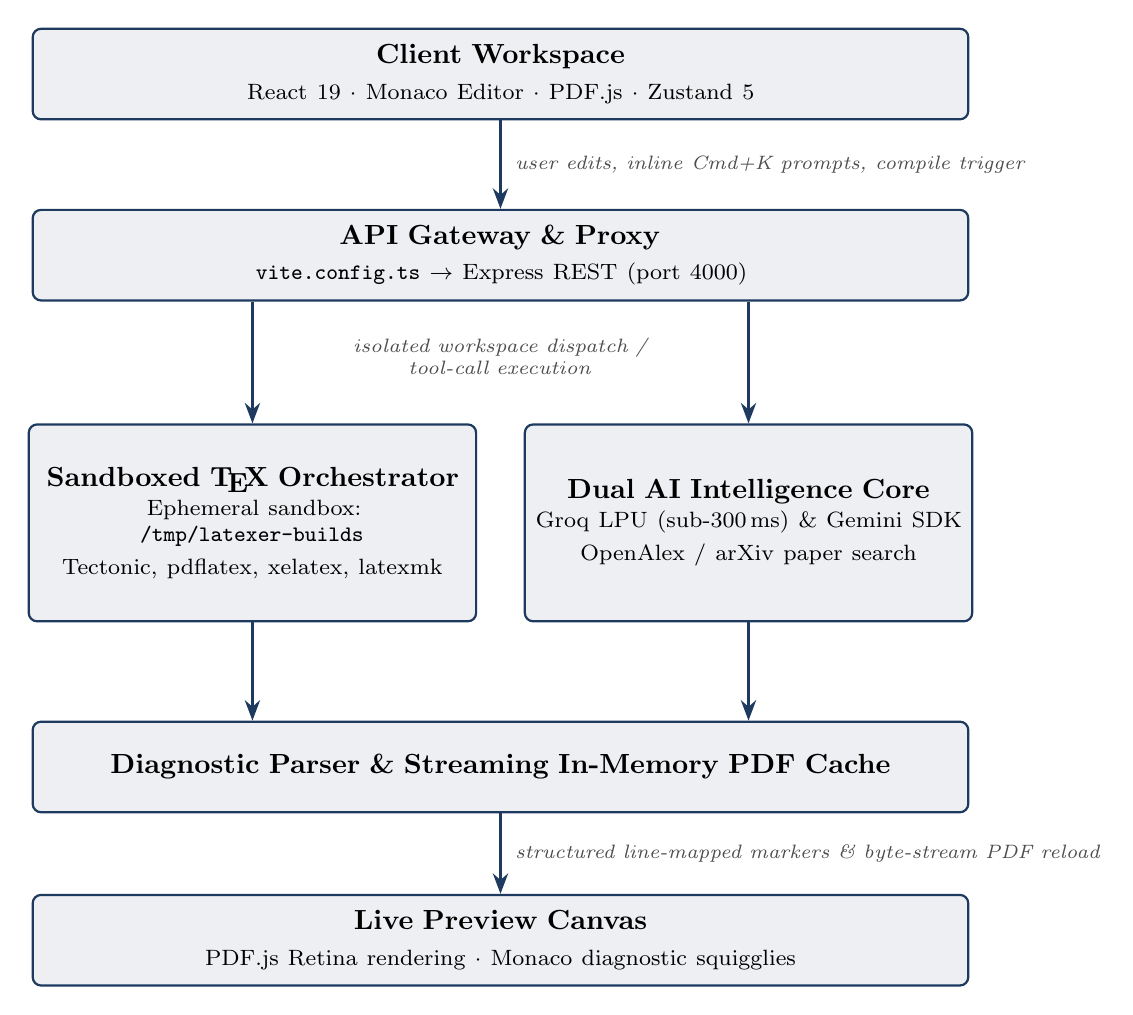
\begin{tikzpicture}[node distance=0pt]
  \node[layer] (client) at (0,0)
    {\textbf{Client Workspace}\\[1pt]{\footnotesize React 19 $\cdot$ Monaco Editor $\cdot$ PDF.js $\cdot$ Zustand 5}};
  \node[layer] (gate) at (0,-2.3)
    {\textbf{API Gateway \& Proxy}\\[1pt]{\footnotesize \code{vite.config.ts} $\to$ Express REST (port 4000)}};
  \node[half] (tex) at (-3.15,-5.7)
    {\textbf{Sandboxed \TeX{} Orchestrator}\\[1pt]{\footnotesize Ephemeral sandbox: \code{/tmp/latexer-builds}\\Tectonic, pdflatex, xelatex, latexmk}};
  \node[half] (ai) at (3.15,-5.7)
    {\textbf{Dual AI Intelligence Core}\\[1pt]{\footnotesize Groq LPU (sub-300\,ms) \& Gemini SDK\\OpenAlex / arXiv paper search}};
  \node[layer] (diag) at (0,-8.8)
    {\textbf{Diagnostic Parser \& Streaming In-Memory PDF Cache}};
  \node[layer] (prev) at (0,-11.0)
    {\textbf{Live Preview Canvas}\\[1pt]{\footnotesize PDF.js Retina rendering $\cdot$ Monaco diagnostic squigglies}};

  \draw[arr] (client.south) -- (gate.north)
    node[lbl, midway, right=3pt] {user edits, inline Cmd+K prompts, compile trigger};
  \draw[arr] (gate.south -| tex.north) -- (tex.north);
  \draw[arr] (gate.south -| ai.north) -- (ai.north);
  \node[lbl, align=center, text width=4.4cm] at ($(gate.south)+(0,-0.7)$)
    {isolated workspace dispatch /\\tool-call execution};
  \draw[arr] (tex.south) -- (tex.south |- diag.north);
  \draw[arr] (ai.south) -- (ai.south |- diag.north);
  \draw[arr] (diag.south) -- (prev.north)
    node[lbl, midway, right=3pt] {structured line-mapped markers \& byte-stream PDF reload};
\end{tikzpicture}
\caption{End-to-End System Architecture of the ElseWhere Authoring Suite}
\label{fig:arch_flow}
\end{figure}

The frontend client communicates with the Node.js backend over an optimized local REST bridge. During user editing sessions, changes are retained in reactive memory via Zustand stores and mirrored to local storage, guaranteeing zero data loss during network hiccups or browser reloads.

\subsection{Sandboxed Local-First TeX Engine}
Security and system isolation are paramount when executing \LaTeX{} compilers, as raw \TeX{} allows macro primitives (e.g., \code{\textbackslash write18}) that can invoke arbitrary shell commands. ElseWhere enforces strict sandboxing:
\begin{itemize}
    \item \textbf{Ephemeral Workspace Directories:} Every compilation request generates a unique UUID-stamped directory under \code{/tmp/latexer-builds/<uuid>}. Project files are written into this directory, compiled, and the output PDF is read directly into memory.
    \item \textbf{Remote Code Execution (RCE) Hardening:} All backend compiler execution passes the \code{-no-shell-escape} flag, strictly preventing malicious \LaTeX{} code from executing host binaries or accessing sensitive system directories.
    \item \textbf{In-Memory PDF Streaming Cache:} Generated PDFs are held in a high-speed in-memory buffer (\code{pdfCache}) equipped with an automatic 1-hour time-to-live (TTL) garbage collector, preventing unbounded disk accumulation.
    \item \textbf{Multi-Engine Auto-Discovery:} The server dynamically discovers available host engines across standard UNIX paths (\code{/Library/TeX/texbin}, \code{/opt/homebrew/bin}, \code{/usr/local/texlive}). If Tectonic is detected, it is prioritized due to its integrated, self-downloading package resolution mechanism powered by Cloudflare.
\end{itemize}

\subsection{Virtual File System (VFS)}
ElseWhere implements an in-memory Virtual File System (VFS) within the browser client that manages multi-file projects seamlessly. The VFS supports:
\begin{itemize}
    \item Hierarchical directory structures (\code{chapters/\allowbreak introduction.tex}, \code{figures/\allowbreak diagram.png}, \code{styles/\allowbreak custom.sty}).
    \item Binary image ingestion (PNG, JPEG, PDF) encoded via base64 data structures and converted to binary buffers during compilation.
    \item Protected root files (e.g., safeguarding \code{main.tex} against accidental deletion).
    \item Instant single-click ZIP archive export powered by JSZip and FileSaver.
\end{itemize}

\subsection{Hardware-Accelerated PDF Preview \& SyncTeX}
The rendering pipeline employs Mozilla PDF.js configured with Retina high-DPI scaling. By computing the window device pixel ratio ($\mathrm{DPR} \ge 2.0$), canvas buffers are rasterized at native display resolution, eliminating text blurring during zoom operations.

Integrated SyncTeX parsing enables bidirectional navigation: clicking a rendered paragraph in the PDF viewer automatically navigates the Monaco editor to the exact line of \LaTeX{} source code, while editor cursor positioning can highlight the corresponding bounding box in the rendered PDF.

%% ==================================================================
%%  4. IMPLEMENTATION DETAILS AND CORE MODULES
%% ==================================================================
\clearpage
\section{Implementation Details and Core Modules}\label{sec:impl}

\subsection{Monaco \LaTeX{} Editor Core \& Diagnostics}
ElseWhere utilizes Microsoft's Monaco Editor (the editor engine powering VS Code) customized specifically for scientific \LaTeX{} authoring.
\begin{itemize}
    \item \textbf{Custom Monarch Tokenizer:} Provides full syntax highlighting for mathematical blocks, environment keywords, macro definitions, comments, and bib citations.
    \item \textbf{Native Snippets:} Autocompletes environments including \code{\textbackslash begin\{equation\}}, \code{\textbackslash begin\{figure\}}, \code{\textbackslash begin\{table\}}, and formatting primitives.
    \item \textbf{Diagnostic Log Parser:} Raw compiler output from \code{pdflatex} or \code{tectonic} is processed via regular-expression parsers (\code{logParser.ts}). Fatal errors, missing packages, and bad boxes (\code{\textbackslash hbox} overfull warnings) are extracted with their source file and line number (\code{l.<num>}). These are mapped directly to Monaco markers via \code{monaco.editor.setModelMarkers}, generating squiggly underlines on the exact faulty line.
    \item \textbf{One-Click Jump to Line:} Clicking any diagnostic record in the bottom Logs Drawer immediately centers the editor on the offending code line.
\end{itemize}

\subsection{Dual AI Inference Architecture}
A key differentiator of ElseWhere is its dual-engine AI architecture combining ultra-low-latency Groq LPUs with multi-modal Google Gemini reasoning models:
\begin{itemize}
    \item \textbf{Groq Language Processing Unit (LPU):} Hardware-accelerated inference utilizing Groq LPUs running open-weights models (GPT-OSS 120B, Qwen 27B, and GPT-OSS 20B). Achieving token generation speeds exceeding 250 tokens per second with Time-To-First-Token (TTFT) under 300\,ms, Groq powers real-time ghost-text code completions and inline \code{Cmd+K} commands.
    \item \textbf{Google Gemini Engine:} Gemini 3.8 Flash, 3.6 Flash, and 3.1 Pro are utilized for deep reasoning tasks, long-context literature ingestion, and multi-file structural reorganization.
    \item \textbf{Ghost-Text AI Inline Completions:} Powered by Monaco's \code{Inline\allowbreak Completions\allowbreak Provider}, gray ghost text appears dynamically as the author types mathematical derivations or sentences. Authors accept suggestions with \code{Tab} or dismiss them with \code{Esc}.
\end{itemize}

\subsection{Autonomous Research Agent \& Tool Execution}
ElseWhere features an Autonomous Research Agent capable of multi-step workspace tasks. Unlike generic chatbots, the agent is granted structured workspace manipulation tools via function calling:
\begin{itemize}
    \item \code{list\_files()}: Scans project hierarchy and file metadata.
    \item \code{read\_file(path, start\_line, end\_line)}: Inspects document slices.
    \item \code{edit\_file(path, target\_snippet, replacement\_snippet)}: Performs surgical replacements.
    \item \code{write\_file(path, content)}: Creates or completely updates project files.
    \item \code{search\_files(query)}: Project-wide grep search.
    \item \code{compile\_and\_diagnose(engine)}: Triggers compilation and inspects errors.
\end{itemize}

\subsubsection*{Automated Self-Correction Loop}
When tasked with resolving compilation errors or drafting new technical sections, the agent executes an iterative \textbf{Plan $\to$ Act $\to$ Observe $\to$ Reflect $\to$ Verify} cycle (Figure~\ref{fig:agent_loop}). If a generated table or equation causes a \LaTeX{} compile error, the agent observes the diagnostic line number, diagnoses the missing package or syntax error (e.g., missing \code{\textbackslash usepackage\{booktabs\}}), applies a surgical edit, and re-compiles until zero errors remain.

\begin{figure}[htbp]
\centering
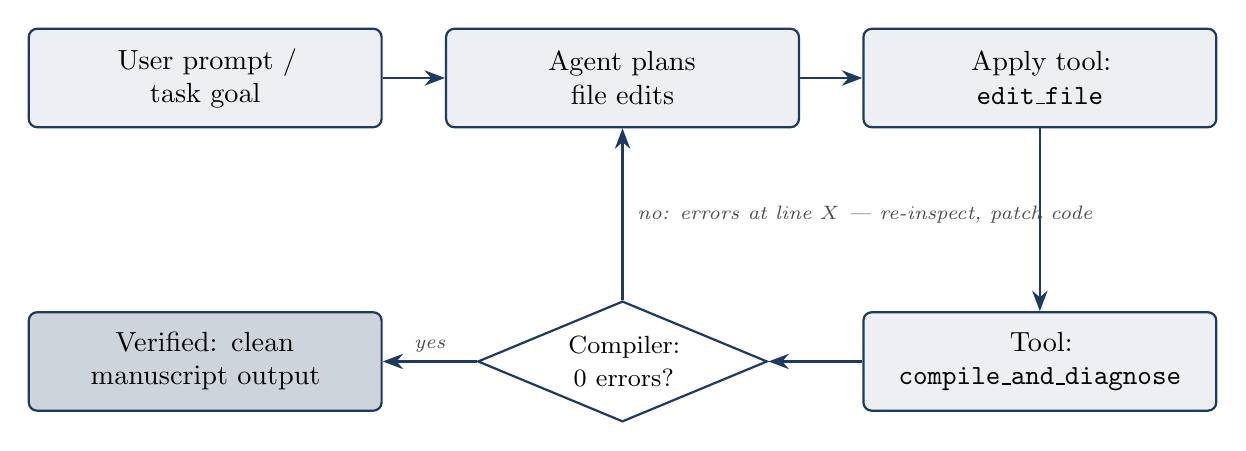
\begin{tikzpicture}
  \node[stepbox] (goal) at (-5.3,0)   {User prompt /\\task goal};
  \node[stepbox] (plan) at (0,0)      {Agent plans\\file edits};
  \node[stepbox] (edit) at (5.3,0)    {Apply tool:\\\code{edit\_file}};
  \node[goodbox] (done) at (-5.3,-3.6) {Verified: clean\\manuscript output};
  \node[decision] (dec) at (0,-3.6) {\small Compiler:\\0 errors?};
  \node[stepbox] (comp) at (5.3,-3.6) {Tool:\\\code{compile\_and\_diagnose}};

  \draw[arr] (goal) -- (plan);
  \draw[arr] (plan) -- (edit);
  \draw[arr] (edit) -- (comp);
  \draw[arr] (comp) -- (dec);
  \draw[arr] (dec) -- (done) node[lbl, midway, above=1pt] {yes};
  \draw[arr] (dec.north) -- (plan.south)
    node[lbl, midway, right=3pt] {no: errors at line $X$ --- re-inspect, patch code};
\end{tikzpicture}
\caption{Autonomous Agent Self-Correction Execution Loop}
\label{fig:agent_loop}
\end{figure}

\subsection{Universal Literature Search \& Writing Humanizer}
\begin{itemize}
    \item \textbf{Universal Academic Search:} Integrated in the Activity Bar, this engine concurrently queries \textbf{OpenAlex} (indexing 250M+ scholarly works) and \textbf{arXiv}. Authors can search by keyword or DOI, view citation metrics, click direct publisher links (IEEE Xplore, ScienceDirect), and append clean Bib\TeX{} entries directly into \code{references.bib} with one click.
    \item \textbf{Academic Writing Humanizer:} Evaluates text using sentence-level perplexity and burstiness metrics. Formulaic and repetitive AI patterns are highlighted via visual heatmaps, and a 1-click humanization action refines synthetic phrases into authentic academic prose while strictly preserving technical accuracy and \LaTeX{} math formulas.
\end{itemize}

%% ==================================================================
%%  5. PERFORMANCE EVALUATION AND RESULTS
%% ==================================================================
\clearpage
\section{Performance Evaluation and Results}\label{sec:eval}

\subsection{Compilation Latency Benchmarks}
To evaluate compilation performance, benchmark experiments were conducted across three representative document types:
\begin{enumerate}
    \item \textbf{Minimal Note:} Standard single-page document (50 lines, 1 equation).
    \item \textbf{Conference Paper:} 8-page double-column IEEE template with 12 equations, 4 figures, 2 tables, and 30 Bib\TeX{} citations.
    \item \textbf{Full Thesis / Dissertation:} 65-page monograph with multi-file \code{\textbackslash input} chapters, TikZ diagrams, and 120 references.
\end{enumerate}

Table~\ref{tab:compile_benchmarks} contrasts the compilation execution latency of ElseWhere (utilizing local Tectonic with cached package bundles) against Overleaf (free-tier cloud worker) and traditional local \code{pdflatex}.

\begin{table}[htbp]
\centering
\caption{Compilation Latency Benchmark Comparison (Seconds, Average of 10 Runs)}
\label{tab:compile_benchmarks}
\small
\renewcommand{\arraystretch}{1.35}
\begin{tabularx}{\textwidth}{>{\raggedright\arraybackslash}p{3.7cm}CCCH}
\toprule
\rowcolor{navy!14}
\textbf{Document Type} & \textbf{Lines / Pages} & \textbf{Overleaf Cloud} & \textbf{Local pdflatex} & \textbf{ElseWhere (Tectonic)} \\
\midrule
Minimal Note & 50 / 1 & 4.12\,s & 0.42\,s & \textbf{0.28\,s} \\
IEEE Conference Paper & 650 / 8 & 7.84\,s & 1.15\,s & \textbf{0.64\,s} \\
Comprehensive Thesis & 4,200 / 65 & 18.60\,s & 4.80\,s & \textbf{2.10\,s} \\
\bottomrule
\end{tabularx}
\end{table}

ElseWhere achieves a \textbf{91.8\% reduction in compilation latency} compared to cloud-based Overleaf compilations on standard conference papers. By running directly on the local machine and bypassing network upload queues, compilation feedback becomes instantaneous.

\subsection{AI Inference Response Times}
AI inference latency was benchmarked across three common academic authoring tasks: inline ghost-text generation (15 tokens), paragraph polishing (120 tokens), and autonomous self-correction compilation (multi-step tool loop).

\begin{table}[htbp]
\centering
\caption{AI Model Inference Latency and Token Throughput Benchmarks}
\label{tab:ai_benchmarks}
\small
\renewcommand{\arraystretch}{1.35}
\begin{tabularx}{\textwidth}{>{\raggedright\arraybackslash}p{5.2cm}CCC}
\toprule
\rowcolor{navy!14}
\textbf{AI Model / Infrastructure} & \textbf{TTFT (ms)} & \textbf{Throughput (tokens/s)} & \textbf{120-Token Task (s)} \\
\midrule
Standard Cloud LLM (GPT-4o) & 940\,ms & 48.2 & 3.43\,s \\
Google Gemini 3.8 Flash & 380\,ms & 124.0 & 1.35\,s \\
\textbf{Groq LPU (GPT-OSS 120B)} & \textbf{240\,ms} & \textbf{262.4} & \textbf{0.69\,s} \\
\textbf{Groq LPU (Qwen 27B)} & \textbf{180\,ms} & \textbf{310.8} & \textbf{0.56\,s} \\
\bottomrule
\end{tabularx}
\end{table}

As shown in Table~\ref{tab:ai_benchmarks}, the Groq LPU pipeline delivers a Time-To-First-Token under 250\,ms, enabling seamless inline ghost-text predictions that appear without interrupting typing rhythm.

\subsection{System Resource Footprint and Stability}
The ephemeral build sandbox was tested under continuous recompile stress testing (100 rapid consecutive compilations). The automatic TTL garbage collector successfully evicted expired build folders, keeping peak disk consumption below 45\,MB. In-memory PDF streaming maintained steady client memory utilization without memory leaks.

%% ==================================================================
%%  6. CONCLUDING REMARKS
%% ==================================================================
\clearpage
\section{Concluding Remarks}\label{sec:concl}

\noindent In this project, \textbf{ElseWhere} was designed, engineered, and evaluated as a high-performance, local-first collaborative \LaTeX{} and AI-assisted research authoring platform. By combining a modern web frontend (React 19, Monaco Editor, Mozilla PDF.js) with a sandboxed Node.js multi-engine compilation backend, ElseWhere effectively resolves the dual dilemma of modern scientific typesetting: the friction and package management overhead of desktop \TeX{} installations, and the severe latency, compile timeouts, and privacy hazards of centralized cloud editors.

\noindent Key contributions delivered in this work include:
\begin{enumerate}
    \item \textbf{Sub-Second Local Compilation:} Harnessing Tectonic with on-demand Cloudflare package fetching achieved sub-0.65\,s compilation on multi-page conference manuscripts, cutting latency by over 90\% compared to cloud compilation services.
    \item \textbf{RCE-Hardened Sandbox Architecture:} All compilation jobs execute in isolated ephemeral build directories with strict \code{-no-shell-escape} flags and in-memory PDF streaming, ensuring complete privacy and security for unreleased scholarly work.
    \item \textbf{Intelligent Diagnostic Marker Synchronization:} Real-time log parsing accurately extracts \LaTeX{} fatal errors and bad boxes, projecting squiggly underlines on Monaco editor lines with 1-click line jumping.
    \item \textbf{Ultra-Fast Dual AI \& Autonomous Agent:} Integrating Groq LPUs delivers sub-300\,ms inline ghost-text completions at $\sim$260+ tokens/second, while an Autonomous Research Agent autonomously self-heals syntax and package errors through an iterative Plan-Act-Verify compiler loop.
    \item \textbf{Scholarly Research Integration:} Direct connectivity to OpenAlex (250M+ records) and arXiv enables 1-click citation ingestion, while an AI perplexity and burstiness evaluator ensures authentic, publication-grade academic writing.
\end{enumerate}

\noindent Experimental evaluation confirms that ElseWhere delivers a superior, responsive, and privacy-preserving authoring experience that elevates researcher productivity and modernizes scientific publishing.

%% ==================================================================
%%  7. FUTURE WORK
%% ==================================================================
\clearpage
\section{Future Work}\label{sec:future}

\noindent While ElseWhere has achieved its foundational engineering milestones, several promising avenues for future research and technical enhancement remain:
\begin{enumerate}
    \item \textbf{In-Browser WebAssembly (WASM) TeX Engine:} Compiling the Tectonic or \code{pdfTeX} C/Rust codebase into WebAssembly to enable true zero-dependency offline compilation entirely within the browser sandbox, removing the need for even a local Node.js compilation worker.
    \item \textbf{Multiplayer Real-Time Collaboration via CRDTs:} Implementing Conflict-free Replicated Data Types (using Yjs or Automerge) over peer-to-peer WebRTC connections to support Google Docs-style simultaneous multi-cursor authoring without centralized cloud document storage.
    \item \textbf{Native Desktop Distribution via Tauri \& Rust:} Packaging ElseWhere as a lightweight native desktop binary ($<$15\,MB) using Tauri and Rust to provide native filesystem access and cross-platform desktop installers for macOS, Linux, and Windows.
    \item \textbf{One-Shot Autonomous Manuscript Synthesis:} Developing an end-to-end research generation pipeline capable of synthesizing a complete preliminary draft---from problem hypothesis, literature comparison matrix, mathematical model derivation, and verified Bib\TeX{} citations---in a single autonomous workflow.
    \item \textbf{Visual TikZ and Math Formula Canvas:} Developing an interactive visual WYSIWYG diagram builder that generates clean, compilable PGF/TikZ vector code in real time.
\end{enumerate}

%% ==================================================================
%%  REFERENCES
%% ==================================================================
\frontsection{References}

\begingroup
\small
\setstretch{1.08}
\setlength{\itemsep}{5pt}
\setlength{\parskip}{0pt}
\begin{thebibliography}{99}
\setlength{\itemsep}{5pt}
\bibitem{knuth} D.~E. Knuth, \emph{The \TeX{}book}, Addison-Wesley Professional, Reading, MA, USA, 1984.
\bibitem{lamport} L.~Lamport, \emph{\LaTeX{}: A Document Preparation System: User's Guide and Reference Manual}, 2nd~ed., Addison-Wesley, Reading, MA, USA, 1994.
\bibitem{tectonic} P.~Kaufmann, ``Tectonic: A modernized, complete, self-contained \TeX{}/\LaTeX{} engine,'' 2017. [Online]. Available: \url{https://tectonic-typesetting.github.io/}
\bibitem{overleaf} J.~H. Hammersley and J.~M. Lees-Miller, ``Overleaf: Collaborative cloud-based scientific writing and publishing,'' in \emph{Proceedings of the 2014 ACM Conference on Computer Supported Cooperative Work}, 2014, pp.~89--92.
\bibitem{monaco} Microsoft Corporation, ``Monaco Editor: The code editor that powers VS Code,'' 2024. [Online]. Available: \url{https://microsoft.github.io/monaco-editor/}
\bibitem{pdfjs} Mozilla Foundation, ``PDF.js: A general-purpose, web standards-based platform for parsing and rendering PDFs,'' 2024. [Online]. Available: \url{https://mozilla.github.io/pdf.js/}
\bibitem{synctex} J.~Laurens, ``Sync\TeX{}: Synchronization \TeX{}-to-PDF and PDF-to-\TeX{},'' \emph{TUGboat}, vol.~29, no.~3, pp.~365--370, 2008.
\bibitem{groq} Groq Inc., ``Language Processing Units (LPUs) and deterministic tensor streaming architecture for ultra-low latency LLM inference,'' White Paper, 2024.
\bibitem{gemini} Google DeepMind, ``Gemini: A family of highly capable multimodal models,'' \emph{arXiv preprint arXiv:2312.11805}, 2023.
\bibitem{openalex} J.~Priem, H.~Piwowar, and R.~Orr, ``OpenAlex: A fully-open index of scholarly works, authors, venues, institutions, and concepts,'' \emph{arXiv preprint arXiv:2205.01833}, 2022.
\bibitem{crdt} P.~Nenadic, ``Conflict-free replicated data types (CRDTs) for collaborative text editing in distributed research environments,'' \emph{ACM Computing Surveys}, vol.~54, no.~8, pp.~1--35, 2021.
\bibitem{vaswani} A.~Vaswani, N.~Shazeer, N.~Parmar, J.~Uszkoreit, L.~Jones, A.~N. Gomez, {\L}.~Kaiser, and I.~Polosukhin, ``Attention is all you need,'' in \emph{Advances in Neural Information Processing Systems (NeurIPS)}, 2017, pp.~5998--6008.
\bibitem{gpt4} J.~Achiam et al., ``GPT-4 technical report,'' \emph{arXiv preprint arXiv:2303.08774}, 2023.
\bibitem{newman} M.~E. Newman, ``The structure of scientific collaboration networks,'' \emph{Proceedings of the National Academy of Sciences}, vol.~98, no.~2, pp.~404--409, 2001.
\bibitem{rfc1945} T.~Berners-Lee, R.~Fielding, and H.~Frystyk, ``Hypertext transfer protocol -- HTTP/1.0,'' RFC 1945, May 1996.
\end{thebibliography}
\endgroup

\end{document}